\documentclass[utf8x, 12pt]{G7-32}

% Настройки стиля ГОСТ 7-32
% Для начала определяем, хотим мы или нет, чтобы рисунки и таблицы нумеровались в пределах раздела, или нам нужна сквозная нумерация.
\EqInChapter % формулы будут нумероваться в пределах раздела
\TableInChapter % таблицы будут нумероваться в пределах раздела
\PicInChapter % рисунки будут нумероваться в пределах раздела
\usepackage{slashbox}

\usepackage[table,xcdraw]{xcolor}

% Добавляем гипертекстовое оглавление в PDF
\usepackage[
bookmarks=true, colorlinks=true, unicode=true,
urlcolor=black,linkcolor=black, anchorcolor=black,
citecolor=black, menucolor=black, filecolor=black,
]{hyperref}

% Изменение начертания шрифта --- после чего выглядит таймсоподобно.
% \usepackage{cyrtimespatched}

% графика
\usepackage{graphicx}
\graphicspath{ {./img/} }

% отделять первую строку раздела абзацным отступом
\usepackage{indentfirst} 

% Пакет Tikz
\usepackage{tikz}
\usetikzlibrary{arrows,positioning,shadows}

% Произвольная нумерация списков.
\usepackage{enumerate}

% ячейки в несколько строчек
\usepackage{multirow}

% itemize внутри tabular
\usepackage{paralist,array}

% объявляем новую команду для переноса строки внутри ячейки таблицы
\newcommand{\specialcell}[2][c]{%
	\begin{tabular}[#1]{@{}c@{}}#2\end{tabular}}

\usepackage{tikz}
\usepackage{pgfplots}
\usepackage{pdfpages}
\usepackage{caption}
% \captionsetup[table]{position=top}
% Листинги

\usepackage{listings}
\usepackage{caption}

\usepackage{courier}
\usepackage{wrapfig}

\usepackage{xcolor}
\captionsetup[lstlisting]{singlelinecheck=off, justification=raggedright}


\definecolor{codegreen}{rgb}{0,0.6,0}
\definecolor{codegray}{rgb}{0.5,0.5,0.5}
\definecolor{codepurple}{rgb}{0.58,0,0.82}
\definecolor{backcolour}{rgb}{0.95,0.95,0.92}


% Значения по умолчанию
\lstset{
  % подсветка синтаксиса
  backgroundcolor=\color{backcolour},   
  commentstyle=\color{codegreen},
  keywordstyle=\color{magenta},
  numberstyle=\tiny\color{codegray},
  stringstyle=\color{codepurple},
  basicstyle= \footnotesize,
  breakatwhitespace=true,% разрыв строк только на whitespacce
  breaklines=true,       % переносить длинные строки
%   captionpos=b,          % подписи снизу -- вроде не надо
  inputencoding=koi8-r,
  numbers=left,          % нумерация слева
  numberstyle=\footnotesize,
  showspaces=false,      % показывать пробелы подчеркиваниями -- идиотизм 70-х годов
  showstringspaces=false,
  showtabs=false,        % и табы тоже
  stepnumber=1,
  tabsize=4,              % кому нужны табы по 8 символов?
  frame=single,
  escapeinside={(*}{*)}, %выделение
  literate={а}{{\selectfont\char224}}1
  {б}{{\selectfont\char225}}1
  {в}{{\selectfont\char226}}1
  {г}{{\selectfont\char227}}1
  {д}{{\selectfont\char228}}1
  {е}{{\selectfont\char229}}1
  {ё}{{\"e}}1
  {ж}{{\selectfont\char230}}1
  {з}{{\selectfont\char231}}1
  {и}{{\selectfont\char232}}1
  {й}{{\selectfont\char233}}1
  {к}{{\selectfont\char234}}1
  {л}{{\selectfont\char235}}1
  {м}{{\selectfont\char236}}1
  {н}{{\selectfont\char237}}1
  {о}{{\selectfont\char238}}1
  {п}{{\selectfont\char239}}1
  {р}{{\selectfont\char240}}1
  {с}{{\selectfont\char241}}1
  {т}{{\selectfont\char242}}1
  {у}{{\selectfont\char243}}1
  {ф}{{\selectfont\char244}}1
  {х}{{\selectfont\char245}}1
  {ц}{{\selectfont\char246}}1
  {ч}{{\selectfont\char247}}1
  {ш}{{\selectfont\char248}}1
  {щ}{{\selectfont\char249}}1
  {ъ}{{\selectfont\char250}}1
  {ы}{{\selectfont\char251}}1
  {ь}{{\selectfont\char252}}1
  {э}{{\selectfont\char253}}1
  {ю}{{\selectfont\char254}}1
  {я}{{\selectfont\char255}}1
  {А}{{\selectfont\char192}}1
  {Б}{{\selectfont\char193}}1
  {В}{{\selectfont\char194}}1
  {Г}{{\selectfont\char195}}1
  {Д}{{\selectfont\char196}}1
  {Е}{{\selectfont\char197}}1
  {Ё}{{\"E}}1
  {Ж}{{\selectfont\char198}}1
  {З}{{\selectfont\char199}}1
  {И}{{\selectfont\char200}}1
  {Й}{{\selectfont\char201}}1
  {К}{{\selectfont\char202}}1
  {Л}{{\selectfont\char203}}1
  {М}{{\selectfont\char204}}1
  {Н}{{\selectfont\char205}}1
  {О}{{\selectfont\char206}}1
  {П}{{\selectfont\char207}}1
  {Р}{{\selectfont\char208}}1
  {С}{{\selectfont\char209}}1
  {Т}{{\selectfont\char210}}1
  {У}{{\selectfont\char211}}1
  {Ф}{{\selectfont\char212}}1
  {Х}{{\selectfont\char213}}1
  {Ц}{{\selectfont\char214}}1
  {Ч}{{\selectfont\char215}}1
  {Ш}{{\selectfont\char216}}1
  {Щ}{{\selectfont\char217}}1
  {Ъ}{{\selectfont\char218}}1
  {Ы}{{\selectfont\char219}}1
  {Ь}{{\selectfont\char220}}1
  {Э}{{\selectfont\char221}}1
  {Ю}{{\selectfont\char222}}1
  {Я}{{\selectfont\char223}}1
}

\lstloadlanguages{
  C++
}

% Стиль для псевдокода: строчки обычно короткие, поэтому размер шрифта побольше
\lstdefinestyle{pseudocode}{
  basicstyle=\small,
  keywordstyle=\color{black}\bfseries\underbar,
  language=Pseudocode,
  numberstyle=\footnotesize,
  commentstyle=\footnotesize\it
}

% Стиль для обычного кода: маленький шрифт
\lstdefinestyle{realcode}{
  basicstyle=\scriptsize,
  numberstyle=\footnotesize
}

% Стиль для коротких кусков обычного кода: средний шрифт
\lstdefinestyle{simplecode}{
  basicstyle=\footnotesize,
  numberstyle=\footnotesize
}

% Стиль для BNF
\lstdefinestyle{grammar}{
  basicstyle=\footnotesize,
  numberstyle=\footnotesize,
  stringstyle=\bfseries\ttfamily,
  language=BNF
}

% Определим свой язык для написания псевдокодов на основе Python
\lstdefinelanguage[]{Pseudocode}[]{Python}{
  morekeywords={each,empty,wait,do},% ключевые слова добавлять сюда
  morecomment=[s]{\{}{\}},% комменты {а-ля Pascal} смотрятся нагляднее
  literate=% а сюда добавлять операторы, которые хотите отображать как мат. символы
    {->}{\ensuremath{$\rightarrow$}~}2%
    {<-}{\ensuremath{$\leftarrow$}~}2%
    {:=}{\ensuremath{$\leftarrow$}~}2%
    {<--}{\ensuremath{$\Longleftarrow$}~}2%
}[keywords,comments]

% Свой язык для задания грамматик в BNF
\lstdefinelanguage[]{BNF}[]{}{
  morekeywords={},
  morecomment=[s]{@}{@},
  morestring=[b]",%
  literate=%
    {->}{\ensuremath{$\rightarrow$}~}2%
    {*}{\ensuremath{$^*$}~}2%
    {+}{\ensuremath{$^+$}~}2%
    {|}{\ensuremath{$|$}~}2%
}[keywords,comments,strings]

% Подписи к листингам на русском языке.
\renewcommand\lstlistingname{\cyr\CYRL\cyri\cyrs\cyrt\cyri\cyrn\cyrg}
\renewcommand\lstlistlistingname{\cyr\CYRL\cyri\cyrs\cyrt\cyri\cyrn\cyrg\cyri}



\begin{document}

\frontmatter % выключает нумерацию ВСЕГО; здесь начинаются ненумерованные главы: реферат, введение, глоссарий, сокращения и прочее.

\begin{table}[ht]
	\centering
	\begin{tabular}{|c|p{400pt}|} 
	\hline
		\begin{tabular}[c]{@{}c@{}} 
\includegraphics[scale=0.37]{EmblemBMSTU} \\\end{tabular} &
		\footnotesize\begin{tabular}[c]{@{}c@{}}\textbf{Министерство~науки~и~высшего~образования~Российской~Федерации}\\\textbf{Федеральное~государственное~бюджетное~образовательное~учреждение}\\\textbf{~высшего~образования}\\\textbf{«Московский~государственный~технический~университет}\\\textbf{имени~Н.Э.~Баумана}\\\textbf{(национальный~исследовательский~университет)»}\\\textbf{(МГТУ~им.~Н.Э.~Баумана)}\\\end{tabular}  \\
	\hline
	\end{tabular}
\end{table}
\noindent\rule{\textwidth}{4pt}
\noindent\rule[14pt]{\textwidth}{1pt}
\hfill 
\noindent
\makebox{ФАКУЛЬТЕТ~}%
\makebox[\textwidth][l]{\underline{~~~~«Информатика и системы управления»~~~~~~~~~~~~~~~~~~~~~~~~~~~~~~~~~~~~~~~~~~~~}}%
\\
\noindent
\makebox{КАФЕДРА~}%
\makebox[\textwidth][l]{\underline{~~~~~~~«Программное обеспечение ЭВМ и информационные технологии»~~~~~~~~}}%
\\


\begin{center}
	\vspace{3cm}
	{\bf\huge Отчёт\par}
	{\bf\Large по лабораторной работе № 2\par}
	\vspace{0.5cm}
\end{center}


\noindent
\makebox{\large{\bf Название:}~~~}
\makebox[\textwidth][l]{\large\underline{~Алгоритмы умножения матриц~~~~~~~~~~~~~}}\\

\noindent
\makebox{\large{\bf Дисциплина:}~~~}
\makebox[\textwidth][l]{\large\underline{~Анализ алгоритмов~~~~~~~~~~~~~~~~~~~~~~~~~~~~~~~~~~~~~~~~~~~~~~~~~~~~}}\\

\vspace{1.5cm}
\noindent
\begin{tabular}{l c c c c c}
    Студент      & ~ИУ7-55Б~               & \hspace{3.5cm} & \hspace{3.5cm}                 & &  Д.Р.Жигалкин \\\cline{2-2}\cline{4-4} \cline{6-6} 
    \hspace{3cm} & {\footnotesize(Группа)} &                & {\footnotesize(Подпись, дата)} & & {\footnotesize(И.О. Фамилия)}
\end{tabular}

\vspace{1cm}

\noindent
\begin{tabular}{l c c c c}
    Преподователь & \hspace{6cm}   & \hspace{3.5cm}                 & & Л.Л. Волкова \\\cline{3-3} \cline{5-5} 
    \hspace{3cm}  &                & {\footnotesize(Подпись, дата)} & & {\footnotesize(И.О. Фамилия)}
\end{tabular}

\begin{center}	
	\vfill
	\large \textit {Москва, 2020}
\end{center}

\thispagestyle {empty}
\pagebreak

\tableofcontents
\pagebreak

\Introduction    
    Умножение матриц -- это одна из самых распространённых опереций над матрицами,
    которая широко применяется в различных численных методах, например, в приложениях 
    для решения системы линейных алгебраических уравений, в программах для 
    преобразований графических структур данных и многих других задачах.

    В данной работе требуется изучить и применить три алгоритма умножения матриц:
    \begin{enumerate}
        \item стандартный алгоритм умножения матриц;
        \item алгоритм Винограда;
        \item оптимизированный алгоритм Винограда.
    \end{enumerate}

    Цель лабораторной работы -- провести сравнительный анализ алгоритмов умножения матриц
    и получить навыки оптимизации трудоёмкости алгоритмов.

    В лабораторной работе ставятся следующие задачи:
     \begin{enumerate}
         \item дать математическое описание формул расчёта умножения матриц для стандарного алгоритма и Винограда;
         \item разработать оптимизированный алгоритм Винограда;
         \item реализовать стандартный алгоритм умножения матриц, Винограда и оптимизированного Винограда;
         \item дать теоритическую оценку трудоёмкости трёх алгоритмов;
         \item провести замеры процессорного времени работы реализаций трёх алгоритмов в худшем и в лучшем случаях.
     \end{enumerate}

\newpage

\mainmatter % это включает нумерацию глав и секций в документе ниже

\chapter{ Аналитический раздел}
\label{cha:analytical}
    В данном разделе будут рассмотрены основные теоритические понятия алгоритмов сортировок
    пузырьком с флагом, вставками, выбором.

    \section{Алгоритмы сортировок}
        \subsection{ Алгоритм сортировки пузырьком с флагом}
            Алгоритм сортировки пузырьком или метод простых обменов имеет следующий 
            принцип работы:
            \begin{enumerate}
                \item прохождение по всему массиву;
                \item сравнивание между собой пар соседних ячеек;
                \item если при сравнении оказывается, что значение ячейки i больше, чем значение ячейки i + 1,
                то нужно поменять значения этих ячеек местами.
            \end{enumerate}

            Алгоритм сортировки пузырьком с флагом является модификацией этого алгоритма.
            Идея состоит в том, что если при выполнении прохода методом пузырька не 
            было ни одного обмена элементов массива, то это означает, что массив уже
            отсортирован и остальные проходы не требуются.

        \subsection{ Алгоритм сортировки вставками}
            Алгоритм сортировки вставками, просматривает элементы входной последовательности по одному,
            и для каждого элемента, размещает его в подходящее место среди ранее упорядоченных элементов.
            
            В начальный момент времени отсортированная последовательность пуста. 
            На каждом шаге алгоритма выбирается один из элементов входных данных и
            помещается в нужную позицию в отсортированной последовательности до тех пор,
            пока набор входных данных не будет исчерпан. 
            
            Сортировка методом вставок -- простой алгоритм сортировки. 
            Хотя этот метод сортировки намного менее эффективен,
            чем более сложные алгоритмы (такие как быстрая сортировка), у него есть ряд преимуществ
            \begin{enumerate}
                \item простота реализации;
                \item эффективен на небольших наборах данных;
                \item эффективен на частично отсортированных последовательностях;
                \item является устойчивым алгоритмом (не меняет порядок элементов, которые уже отсортированы).
            \end{enumerate}

            Данный алгоритм можно ускорить при помощи использования бинарного поиска для нахождения места
            вставки текущего элемента в отсортированную часть последовательности.

        \subsection{ Алгоритм сортировки выбором}
            Алгоритм сортировки выбором работает следующим образом: 
            находим наименьший элемент в массиве и обмениваем его с элементом находящимся на первом месте.
            Повторяем процесс -- находим наименьший элемент в последовательности, начиная со второго элемента, и
            обмениваем со вторым элементном и так далее, пока весь массив не будет отсортирован.
            Этот метод называется сортировка выбором, поскольку он работает, 
            циклически выбирая наименьший из оставшихся элементов.

            Главным отличием сортировки выбором от сортировки вставками является, то что в сортировке вставками 
            извлекается из неотсортированной части массива первый элемент (не обязательно минимальный) и
            вставляется на своё место в отсортированной части.
            В отличии от сортировки выбором, где ищется минимальный элемент 
            в неотсортированной части,  который вставляется в конец отсортированной части массива.


    \section{Трудоёмкость алгоритма}
        Трудоёмкость -- количество работы, которую алгоритм затрачивает на обработку данных.
        Является функцией от длины входов алгоритма и позволяет оценить количество работы.

        Введём модель вычисления трудоёмкости.

        \subsection{Базовые операции}
            Ниже представлены базовые операции, стоимость которых единична:
            \begin{enumerate}
                \item $ =, +, +=, -, -=, *, *=,  /, /=, ++, --, \% $,
                \item $ <, \leqslant, ==, \neq, \geqslant , > $,
                \item $ [ $  $ ] $.
            \end{enumerate}
            
        \subsection{Условный оператор}
            if (условие) \{

                // тело A

            \}

            else \{

                // тело B
            
            \}

            Пусть трудоёмкость тела A равна $ f_A $, а тела B $ f_B $, тогда
            стоимость условного оператора можно найти по формуле (\ref{equation:trud:if}):
            \begin{equation}
                f_{if} = f_\text{условия} + \left\{
                    \begin{matrix}
                    min(f_A, f_B) - \text{лучший случай},\\
                    max(f_A, f_B) - \text{худший случай} 
                    \end{matrix}\right.
                \label{equation:trud:if}
            \end{equation}

        \subsection{Цикл со счётчиком}
            for (int i = 0; i < n; i++) \{

                // тело цикла

            \}
            
            Начальная инициализация цикла (int i = 0) выполняется один раз.
            Условие i < n проверяется перед каждой итерацией цикла и при входе в цикл -- n + 1 операций.
            Тело цикла выполняется ровно n раз.
            Счётчик (i++) выполняется на каждой итерации, перед проверкой условия, т.е. n раз.
            Тогда, если трудоёмкость тела цикла равна $ f $, трудоёмкость всего цикла определяется формулой (\ref{equation:trud:for})

            \begin{equation}
                f_\text{цикла} = 2 + n(2 + f)
                \label{equation:trud:for}
            \end{equation}
\newpage
\chapter{ Констукторский раздел}
\label{cha:design}
    В данном разделе будет рассмотрена схема алгоритма, требования к функциональности ПО,
    и опредены способы тестирования.
    
    \section{Разработка алгоритма}
        Ниже будет представлена схема алгоритма обратной трассировки лучей.

        Алгоритм обратной трассировки лучей (рисунок \ref{schema:rtx});


    \begin{figure}[h!]
        \centering
            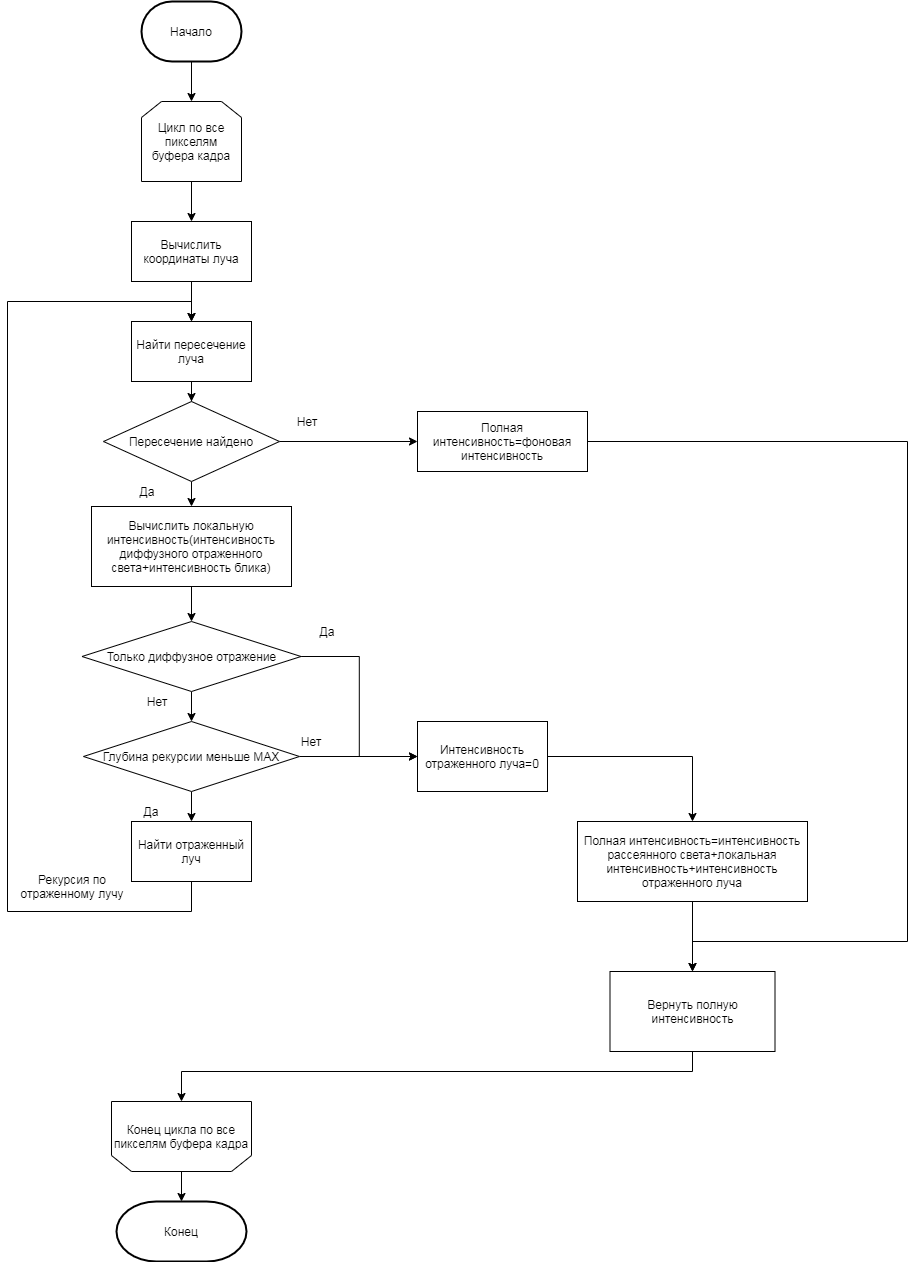
\includegraphics[scale=1.0]{rtx.png}
            \caption{Схема алгоритма обратной трассировки лучей}
            \label{schema:rtx}
    \end{figure}

    \section{Параллельные вычисления}
Распрараллеливание программы должно ускорять время работы. Это достигается за счет реализации в узких участках (напимер в циклах с большим количеством независимых вычилений).

В предложенном алгоритме данным участком будет являться основной двойной цикл вычислений.
Данный блок программы как раз предлагается распараллелить.


    \section{Требования к функциональности ПО}
        В данной работе требуется обеспечить следующую минимальную функциональность оконного приложения:
        \begin{enumerate}
	\item обеспечить ввод координат положения камеры наблюдателя;
	\item обеспечить ввод значения угла, на который необходимо повернуть камеру наблюдателя относительно оси oY;
            \item обеспечить вывод полученного с помощью алгоритма обратной трассировки лучей изображения;
            \item обеспечить вывод замеров времени работы алгоритма обратной трассировки лучей.
        \end{enumerate}

    \section{Методы тестирования}
    Тестирование ПО будет проводиться методом черного ящика.

\newpage
\chapter{ Технологический раздел}
\label{cha:technological}

    В данном разделе будут выбраны средства реализации ПО и представлен листинг кода. 

    \section{Средства реализации}
        В данной работе используется язык программирования C\# \cite{Charp}, так как
        он позволяет написать программу в относительно малый срок.
        В качестве среды разработки использовалась Visual Studio 2017. \cite{visual-studio}

        Для замера процессорного времени был использован класс Stopwatch. \cite{stopwatch}

	Многопоточное программирование было реализовано с помощью пространства имен System.Threading. \cite{thread}


        \begin{lstlisting}[label=lst:rtx_parall, caption=Реализация алгоритма обратной трассировки лучей с параллельными вычислениями]
            int n = 4; // Количество потоков

            int step = data.Width / n;

            Thread[] t = new Thread[n];
       
            int x1 = 0;
            int x2 = step;

            int y1 = 0;
            int y2 = data.Height;
         
            for (int i = 0; i < n; i++)
            {
                AllParameters p = new AllParameters(x1, y1, x2, y2);

                t[i] = new Thread(Process);
                t[i].Start(p);

                x1 = x2;
                x2 += step; 
            }

            foreach (Thread thread in t)
            {
                thread.Join();
            }

            void Process(object obj)
            {
                AllParameters p = (AllParameters)obj;

                int x = p.x;
                int y = p.y;

                int endx = p.endx;
                int endy = p.endy;

                for (int i = x; i < endx; i++)
                {
                    for (int j = y; j < endy; j++)
                    {
                        int[] work = { i - data.Height / 2, j - data.Width / 2 };

                        double[] direction = RayTracing.CanvasToViewport(data.Width, data.Height, work);
                        direction = MyMath.MultiplyMV(cameraRotationOY, direction);

                        double[] color = RayTracing.TraceRay(recursionDepth, lights, objects, cameraPosition, direction, 1, Double.PositiveInfinity, 0);

                        var offset = ((j * data.Width) + i) * depth;

                        buffer[offset + 0] = (byte)color[2];
                        buffer[offset + 1] = (byte)color[1];
                        buffer[offset + 2] = (byte)color[0];
                    }
                }

            }
        \end{lstlisting}

    

\newpage
\chapter{Экспериментальный раздел}
\label{cha:research}
    В данном разделе будут проведены эксперименты для проведения 
    сравнительного анализа трёх алгоритмов по затрачиваемому процессорному 
    времени в зависимости от размеров матриц и чётности / нечётности размеров.

    \section{Сравнительный анализ на основе замеров времени работы алгоритмов}
        В рамках данного проекта были проведёны следующие эксперименты:
        \begin{enumerate}
            \item сравнение времени работы алгоритмов на размерностях квадратных матриц 100, 200, 300, 400, 500 (график \ref{graph:test:1});
            \item сравнение времени работы алгоритмов на размерностях квадратных матриц 101, 201, 301, 401, 501 (график \ref{graph:test:2}).
        \end{enumerate}

        Матрицы заполнялись случайными числами.

        Тестирование проводилось на ноутбуке с процессором
        Intel(R) Core(TM) i5-7200U CPU 2.50 GHz \cite{processor-i5-7200u}
        под управлением Windows 10 с 8 Гб оперативной памяти.

        В ходе экспериментов по замеру времени работы было установлено, что 
        оптимизированный алгоритм Винограда быстрее неоптимизированого при больших размерностях матриц , в частности, на 43 \% и
        на 14-20 \% при размере матрицы 400 стандартного в зависимости от чётности совпадающей размерности матриц.  Оптимизированный алгоритм 		Винограда также быстрее стандратного алгоритма Винограда при больших размерностях матрицы.


    \begin{figure}[h!]
        \centering
        \begin{tikzpicture}
            \begin{axis}[
                legend pos = north west,
                grid = major,
                xlabel = Размер матрицы,
                ylabel = {Время, сек},
                height = 0.5\paperheight, 
                width = 0.75\paperwidth
            ]
            
            \addplot table[x=n,y=std] {data/test1.dat};
            \addplot table[x=n,y=vin] {data/test1.dat};
            \addplot table[x=n,y=optVin] {data/test1.dat};
            \legend{
                Стандартный алгоритм,
                Алгоритм Винограда,
                оптимизированный алгоритм Винограда,
            };
            \end{axis}
        \end{tikzpicture}
        \caption{График зависимости времени работы алгоритмов при чётных размерностях матриц} 
        \label{graph:test:1}
    \end{figure}

    \begin{figure}[h!]
        \centering
        \begin{tikzpicture}
            \begin{axis}[
                legend pos = north west,
                grid = major,
                xlabel = Размер матрицы,
                ylabel = {Время, сек},
                height = 0.5\paperheight, 
                width = 0.75\paperwidth
            ]
            
            \addplot table[x=n,y=std] {data/test2.dat};
            \addplot table[x=n,y=vin] {data/test2.dat};
            \addplot table[x=n,y=optVin] {data/test2.dat};
            \legend{
                Стандартный алгоритм,
                Алгоритм Винограда,
                оптимизированный алгоритм Винограда,
            };
            \end{axis}
        \end{tikzpicture}
        \caption{График зависимости времени работы алгоритмов при нечётных размерностях матриц} 
        \label{graph:test:2}
    \end{figure}

\newpage

\backmatter % Здесь заканчивается нумерованная часть документа и начинаются ссылки и
\Conclusion
    В ходе выполнения лабораторной работы были достигнуты следующие задачи:
    \begin{enumerate}
        \item изучен алгоритм обратной трассировки лучей;
        \item реализован алгоритм обратной трассировки лучей;
        \item проведены замеры процессорного времени работы от разного числа параллельных потоков;
        \item проведено сравнение параллельных реализаций алгоритма обратной трассировки лучей со стандартной реализацией.
    \end{enumerate}

В ходе сравнения процессорного времени работы было установлено:
	\begin{enumerate}
	\item параллельная реализация алгоритма обратной трассировки лучей в случае увеличения числа потоков в 2 раза, начиная с 8 замедляет скорость своей работы;
	\item максимальный прирост скорости параллельной реализации алгоритма обратной трассировки лучей достигается при количестве потоков равных 4 и равен  $ \approx 1.7 $ раза.


        \end{enumerate}

Эксперементальным путем было выяснено, что увеличение количества потоков в 2 раза не всегда увеличивает производительность программы.

    


\bibliographystyle{gost780u}
\bibliography{report}

\end{document}